\documentclass[11pt,titlepage,oneside]{book}
\usepackage{graphicx}
\graphicspath{ {./images/} }
\usepackage[lmargin=1in,rmargin=1in,tmargin=1in,bmargin=1in]{geometry} % see geometry.pdf on how to lay out the page. There's lots.
\geometry{a4paper}

%%%%%%%%%%%%%%%%% PACKAGES %%%%%%%%%%%%%%%%%

\usepackage{graphicx} % enhanced grpahics support
\renewcommand{\sfdefault}{cmbr} % slightly nicer than the standard sans serif font
\usepackage[onehalfspacing]{setspace} % line spacing
\usepackage[T1]{fontenc} % font encoding (fixes some font-related errors)
\usepackage{textcomp} % more font encoding
\usepackage[printonlyused]{acronym} % To handle acronyms
\usepackage{appendix} % For managing appendices (makes ToC neater)


%%%%%%%%%%%%%%%%% DOCUMENT PROPERTIES %%%%%%%%%%%%%%%%%

% Thesis details
\newcommand{\LongTitle}{My Technical Progress Project}
\newcommand{\Me}{Harvey Prewer}

% Number of document levels
\setcounter{secnumdepth}{4}

% Prevent hyphenation
\hyphenpenalty=5000
\tolerance=1000

%%%%%%%%%%%%%%%%% ACRONYMS AND SYMBOLS %%%%%%%%%%%%%%%%%

\newcommand{\RT}{RT\ensuremath{_{\text{60}}}}
\newcommand{\DEG}{\ensuremath{^\circ}}

%%%%%%%%%%%%%%%%% DATE %%%%%%%%%%%%%%%%%

% For placing on title page
\usepackage{datetime}
\newdateformat{MyMonth}{\monthname[\THEMONTH]}
\newdateformat{MyYear}{\THEYEAR}
\newdateformat{MyDate}{\THEYEAR}

%%%%%%%%%%%%%%%%% CAPTIONS %%%%%%%%%%%%%%%%%

\usepackage[margin=2em,singlelinecheck=on,font=sf,labelfont+=bf,labelformat=simple,labelsep=colon]{caption}

\newcommand{\captionfontsize}{\fontsize{9}{11}\selectfont}
\renewcommand\captionfont{\captionfontsize\sffamily}

\bibliographystyle{iosrnew.bst}


%%%%%%%%%%%%%%%%% TITLES %%%%%%%%%%%%%%%%%

\usepackage[sf,raggedright,toctitles]{titlesec}

% Chapter heading properties
\titlespacing{name=\chapter}{0ex}{0ex}{.5in}[0ex]
\titlespacing{name=\chapter,numberless}{0ex}{0ex}{.5in}[0ex]

% Subsubsection heading properties
\titleformat{name=\subsubsection,numberless}[hang]{\sf}{}{0pt}{\bfseries}
\titlespacing{name=\subsubsection,numberless}{0em}{2ex}{0ex}

%%%%%%%%%%%%%%%%% TOC / LOF / LOT / LOE %%%%%%%%%%%%%%%%%

\usepackage[titles]{tocloft}

\setcounter{lofdepth}{1}

% put "Chapter #: " in ToC
\renewcommand{\cftchappresnum}{\chaptername~}
\renewcommand{\cftchapaftersnum}{:}
\newlength{\mylen} % a "scratch" length
\settowidth{\mylen}{\bfseries\chaptername\cftchapaftersnum} % extra space
\addtolength{\cftchapnumwidth}{\mylen} % add the extra space

% control indention
\setlength{\cftchapindent}{0em}
\setlength{\cftfigindent}{0em}
\setlength{\cfttabindent}{0em}

\newlength{\tocloftindent}
\setlength{\tocloftindent}{2.3em}

\setlength{\cftsecindent}{1.5em}

%\renewcommand{\@pnumwidth}{1.9em} % was 1.55em
%\renewcommand{\@tocrmarg}{2.9em plus1fil} % raggedright toc entries (no hyphenation)

\setlength{\cftsubsecindent}{3.8em}

%%%%%%%%%%%%%%%%% TABLES %%%%%%%%%%%%%%%%%

\usepackage{array,color,colortbl,multirow,longtable}

\newcommand{\colheading}[1]{\multirow{2}{*}{\textbf{#1}}} % custom column heading command
\newcommand{\tablesubtitle}[2]{\multicolumn{#1}{l}{\emph{#2}}} % custom table sub heading to span the specified number of columns
\renewcommand\arraystretch{1.2} % row height

%%%%%%%%%%%%%%%%% MATHS %%%%%%%%%%%%%%%%%

\usepackage{amsmath,amsbsy,amssymb}

\allowdisplaybreaks

% define new symbols and operators
\newcommand{\R}{\mathfrak{R}} % Real operator
\newcommand{\Z}{\mathbb{Z}} % set of integers
\newcommand{\N}{\mathbb{N}} % set of natural numbers
\newcommand{\F}{\mathcal{F}} % Fourier operator
\newcommand{\ud}{\,\text{d}} % d in differential
\newcommand{\fs}{f\negthinspace{}s} % sampling frequency
\DeclareMathOperator*{\argmax}{arg\,max} % arg min
\DeclareMathOperator*{\argmin}{arg\,min} % arg max
\providecommand{\abs}[1]{\lvert#1\rvert} % abs brackets

%%%%%%%%%%%%%%%%% CITATIONS %%%%%%%%%%%%%%%%%

\usepackage[round]{natbib}
\setcitestyle{aysep={ },notesep={: },citesep={;},yysep={,}}

\setlength{\bibhang}{0pt}

\newcommand{\citepos}[1]{\citeauthor{#1}'s \citeyearpar{#1}}
\newcommand{\citequote}[1]{\newline \strut\hfill \citep{#1}}
\newcommand{\cpage}[1]{p.~#1}
\newcommand{\cpages}[2]{pp.~#1--#2}
\renewcommand\bibname{References}

%%%%%%%%%%%%%%%%% HEADER/FOOTER %%%%%%%%%%%%%%%%%

\usepackage{fancyhdr}
\setlength{\headheight}{15pt}

\newcommand{\myfooter}{\textsf{\thepage}}

\fancypagestyle{plain}{%
	\fancyhf{}%
	\fancyfoot[R]{\myfooter}%
	\renewcommand{\headrulewidth}{0pt}%
	\renewcommand{\footrulewidth}{1pt}%
}

\pagestyle{fancy}
\fancyhf{}%
\renewcommand{\headrulewidth}{1pt} %header line width
\renewcommand{\footrulewidth}{1pt} % footer rule width
\fancyhead[R]{\textsf{\nouppercase{\leftmark}}} % header right - chapter title
\fancyfoot[R]{\myfooter} % footer right - page number

%%%%%%%%%%%%%%%%% HYPERREF %%%%%%%%%%%%%%%%%

% this should hopefully be the last entry in the preamble - defines properties of the typeset pdf file
% this package makes clickable links in the pdf
\usepackage[colorlinks,pdftex,breaklinks,pdfdisplaydoctitle,plainpages=false]{hyperref} 
\hypersetup{pdftitle={\LongTitle},pdfauthor={\Me},
	citecolor=black,%
	filecolor=black,%
	linkcolor=black,%
	urlcolor=black
}

\renewcommand{\equationautorefname}{Equation}
\renewcommand{\figureautorefname}{Figure}
\renewcommand{\Itemautorefname}{Item}
\renewcommand{\tableautorefname}{Table}
\renewcommand{\sectionautorefname}{Section}
\renewcommand{\subsectionautorefname}{Section}
\renewcommand{\subsubsectionautorefname}{Section}
\renewcommand{\chapterautorefname}{Chapter}
\renewcommand{\partautorefname}{Part}


\title{Tech Project Progress Report}
\author{Harvey Prewer}

\begin{document}

\begin{titlepage}

\thispagestyle{empty}
\hfill\includegraphics[width=50mm]{UniS_Logo.pdf}
{\sf
	\centering
	\null\vfil\vfil
	{
		\huge\LongTitle\\
	}
	\vfil\vfil\vfil
	{
		\Large\Me\\
	}
	\vfil\vfil\vfil
	{
		\Large{}BMus/BSc Music \& Sound Recording (Tonmeister)\\
		Technical Project\\
	}
	\vfil\vfil
	{
		\Large{}Institute of Sound Recording\\
		University of Surrey\\
	}
	\vfil
	{
		\Large\MyMonth\today~\MyYear\today\\}
}

{
	\includegraphics[width=40mm]{University_of_Surrey_coat_of_arms.pdf}
	\vspace{-.4in}
}

\end{titlepage}
\section{Introduction}
	 \begin{flushleft}
	 Few options exist for algorithmically finding song recommendations for DJ sets. Building a DJ set by manually searching for songs is very time consuming, so improved, automated, recommendation systems would make this process more efficient . 
	\end{flushleft}

\begin{flushleft}
	 The music recommendation application would cater for professional and aspiring DJs, and music lovers drawn to radio and DJ sets. The application will take a DJ set identifier as input and output song recommendations. The recommendation algorithm will use collaborative filtering or content based filtering, with MixesDB as the source dataset. It will be implemented as a python console application.
	\end{flushleft}
\section{Potential Methods}
	 \subsection{Collaborative-Based Filtering}
	 \begin{enumerate}
	 	
	 	\item  Input a DJ Setlist to a matrix with the number of plays a song has by a given DJ.
	 	\item The program looks over DJs who played the songs included in the set, removing from the MixesDB data any tracks that are already in the input DJ set.
	 	\item Added weight on DJs who've played the most significant majority of songs on the mix, allowing other songs played by them to make up the majority of the recommendations.
	 \end{enumerate}
  \subsection{Content-Based Filtering}
  To implement Content Based Filtering, you would need to:
 \begin{enumerate}
 	
 	\item  Profile the features of all the tracks in MixesDB. Some of these features would need to come from Spotify, as per the medium article. Features specific to your application would be the DJ and/or number of DJs who have played the track and the number of sets the track appears in.
 	
 	\item For each track, the features would be converted into a vector.
 	
 	\item Take the input DJ Set, that you're recommending for and repeat the same feature analysis as above. The result would be a vector track, which could then be summarised into a single vector for the whole set.
 	
 \end{enumerate}

\section{Motivation}

	The hypothesis is that the application will give song recommendations that are both stylistically suitable but aren't necessarily popular (a common trait in most recommendation systems), because of the characteristics of a DJ set. For example, a typical quality of DJ sets is the great lengths the DJ goes to find obscure and unknown songs. Therefore, not prioritising popularity is a desirable trait in a recommendation system for a DJ's music consumption and knowledge, usually being more than the average consumer. 
	
	\begin{flushleft}
		
		A DJ set can also be described as musical recommendations curated by a person passionate enough about music to make selecting and playing songs their profession or a well-invested hobby. I want to explore if creating a music recommendation system that builds from archives of these personally selected songs would create a pool of more "human" suggestions than what Spotify or other streaming platforms recommends. Another benefit is that what a DJ plays is not limited to a specific format, so my application suggests music on all platforms.
		
	\end{flushleft}
	
	
\section{Research Questions}
	\subsection{What are the effective methods of automating the recommendation for suitable songs added to a given DJ set?}
	
	I see the need for this application due to how laborious it is to look for songs from DJ sets you like. Discovering new music from DJ sets includes endlessly digging through the DJs, Artists, Labels and Genres associated with the mix, which is very time-consuming. 
	
	\begin{flushleft}
		The lack of recommendation systems for DJ sets makes this application more noteworthy. Besides manually finding songs, I have discovered two inadequate ways of getting recommendations based on DJ sets:
	\end{flushleft}
	
	\begin{enumerate}
		
		\item \textbf{Spotify }- Find a DJ set on Spotify (not commonly available but labels like !K7 Music releases DJ sets commercially as albums), add that to a playlist, and look at the" Recommended based on the playlist". The main problem with this is that DJ sets on Spotify are few and far between. One can only input a mix one's heard from the radio or a recorded live performance by finding the tracklist and adding the songs into a playlist. The system also finds what other users are listening to, often giving you song recommendations that are usually quite popular and well-known. Spotify has a vast library of music, but a sizeable chunk of music played on Spotify you won't find on DJ sets. 
		
		\item \textbf{SoundCloud }- When a DJ set gets uploaded to SoundCloud, it usually recommends other DJ sets on its " radio " when getting recommended songs is more desirable. The recommendation system is only limited to what is available on SoundCloud.
	\end{enumerate}

	\subsection{Is this proposed method a suitable solution to the above question?}
	
	The use of collaborative filtering is used a lot in recommendation systems amongst different formats. It first came to prevalence by the winner of the Netflix Prize in 2007 and 2008 using the technique extensively\citep{zhou_large-scale_2008}. In a 2020 medium article, a song recommendation system for DJs used collaborative filtering to find valid suggestions\citep{chow_music_2020}.
	
	\begin{flushleft}
		The advantage content-based filtering has over collaborative filtering is its ability to recommend new and unpopular music, which as mentioned before is desirable for DJs\citep{van_den_oord_deep_2013}.
	\end{flushleft}
	
	
	\subsection{Can this application be further developed to solve other DJ tasks?}
	The application could be developed to aid aspiring DJs in showing songs suitable to mix in and out of songs they already know. The input is a song, and the output is the songs played before or after in other DJ sets.
	
\section{Potential Issues}
A problem will arise when multiple DJs are involved in a DJ set. To solve this, I'll label this DJ set and its track selection as being from both DJs, and this is valid because the fact they are DJing together shows some crossover in taste.

\begin{flushleft}
	Another limitation is that it will only recommend songs from MixesDB. This small dataset may affect the quality of some suggestions.
\end{flushleft}

\begin{flushleft}
	Another issue is how well the level of cohesiveness matches the suggestions. For example, if a set plays a variety of genres, will the pool of recommendations reach that level of diversity? The application should pick DJs that match the input set's cohesion level. If not, the programme could solve this by capping the number of song suggestions from specific DJs. For example, suppose the input DJ set is House, Techno and Rock songs, but the DJ themselves usually just DJs dance music. In that case, this cap will limit the suggestion pool from House and Techno and, hopefully, let a suitable amount of Rock suggestions be selected. 
\end{flushleft}

	
\section{Summary of Literature Review}
\begin{flushleft}
	The literature review will answer the first and last questions in the literature review.
\end{flushleft}
\begin{flushleft}
	The literature review will explore the best methods used for state-of-the-art music song recommendation systems. This chapter will include mentioning collaborative filtering \citep{chow_music_2020}, content-based filtering \citep{chang_building_2021} and clustering\citep{piyush_building_2019}. This part will also discuss the need to use deep learning to expand a recommendation system beyond its database. It will then discuss how a DJ's taste is diverse and diverse listeners are more refrained from using less algorithmic means to find music \citep{anderson_algorithmic_2020}.
\end{flushleft}
\begin{flushleft}
	For the final one, the chapter will discuss other machine learning-aided DJ technologies. An example of this is the source separation stuff found \citep{kirn_review_2023}, and it will discuss whether my proposed method can contribute to the problem the other applications are fixing. Then, it will relate to how my approach can be helpful for other DJ-related necessities. 
\end{flushleft}
\begin{flushleft}
	The readings here will determine the answer to the second research question.
	
\end{flushleft}

\section{Time Plan}

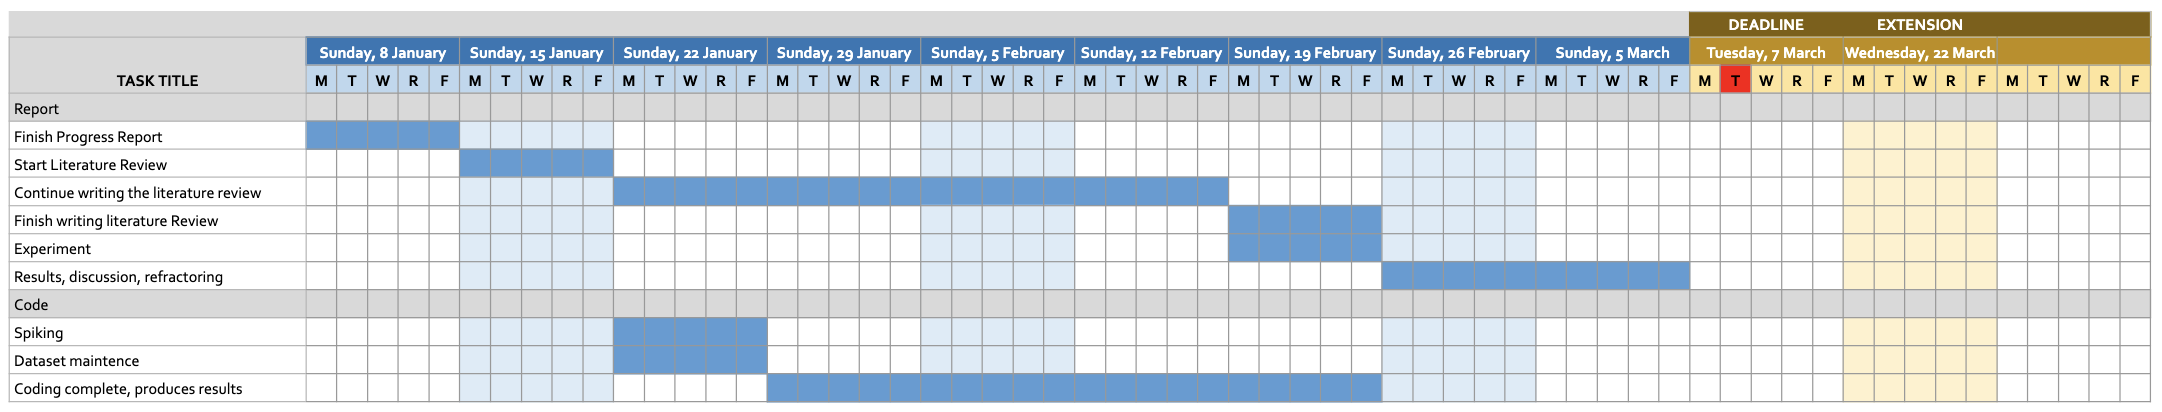
\includegraphics[width=\columnwidth]{timePlan}



\section{Outline Experiment Plan}
Make a python console application that uses collaborative filtering and MixesdB as the source dataset. The input will be a text file of a DJ set you enjoy and the program outputs a text file listing songs similar to the input DJ set.

\begin{flushleft}
	For testing there is got two methods: 
\end{flushleft}
\begin{enumerate}
	\item First is using spectrogram comparisons of different methods. Spectrograms of the songs in the set list and the recommended songs will be taken. Within the recommended songs it will compare itself amongst the songs in the DJ set concluding which one it’s most similar to. Then there will be a discussion about the overall similarity rating of each song and how well distributed it is amongst the inputted DJ set.
	\item After this, backtesting will be used. This is when the songs of a said year is inputted, and looked at the recommendations it gives, and it will then compare the recommendations to the songs that were played in DJ sets the year after. This will be a good indication of whether the songs recommended are ones that a DJ would go out and play.
\end{enumerate}

\section{Chapter Layout of Final Report}
\begin{enumerate}
	\item Chapter 1 Introduction
	\item Chapter 2 - Machine Learning used in Music Recommendation Systems
	\begin{enumerate}
		\item The need for Recommendation Systems
		\item Collaborative Filtering
		\item Content Based Filtering
		\item Clustering
		\item Convoluted Networks
	\end{enumerate}
	\item Chapter 3 - Machine Learning used for DJing
	\begin{enumerate}
		\item Source Separation
		\item BPM, key, genre classification
		\item Beat Tracking 
	\end{enumerate}
	\item Chapter 4 - Hypothesis
	\item Chapter 5 - Experiment
	\item Chapter 6 - Results and Discussion
	\item Chapter 7 - Further Work
	
\end{enumerate}

\bibliography{BackgroundReading.bib}
\end{document}


